\documentclass{article}
\usepackage[utf8]{inputenc}
\usepackage[T1]{fontenc}
\usepackage[export]{adjustbox}
\usepackage{mathtools,amsthm,amssymb,icomma,upgreek,xfrac,enumerate, bbm,titlesec,lmodern,polski,derivative,geometry,multicol,titling,graphicx,url,amsmath,caption,lipsum,float,longtable,booktabs}
\usepackage[table,xcdraw]{xcolor}
\usepackage[hidelinks,breaklinks,pdfusetitle,pdfdisplaydoctitle]{hyperref}
\setlength{\droptitle}{-1cm}
\mathtoolsset{showonlyrefs,mathic}
\title{Komputerowa analiza szeregów czasowych raport 1}
\author{Natalia Klepacka, Joanna Kołaczek}
\date{21.12.2022}
\newtheoremstyle{break}
{\topsep}{\topsep}%
{\normalfont}{}%
{\bfseries}{}%
{\newline}{}%
\theoremstyle{break}
\newtheorem{zadanie}{Zadanie} 
\newtheorem*{rozwiazanie}{Rozwiązanie}

\titleformat*{\section}{\LARGE\bfseries}
\titleformat*{\subsection}{\Large\bfseries}
\titleformat*{\subsubsection}{\large\bfseries}
\titleformat*{\paragraph}{\large\bfseries}
\titleformat*{\subparagraph}{\large\bfseries}

\graphicspath{{obrazki/}}


\begin{document}
	\maketitle
	\tableofcontents
	\clearpage
\section{Wstęp}
	Niniejszy raport powstał na potrzeby realizacji laboratorium z Komputerowej Analizy Szeregów Czasowych, prowadzonych przez mgr Justynę Witulską, do wykładu prof. Agnieszki Wyłomańskiej.
	Będziemy analizować dane dotyczące poziomu szczęścia w wybranych krajach na świecie, oraz dane dotyczące wpływu na szczęście poziomu PKB na osobę (w dalszej części raportu, będziemy je określać skrótowo jako szczęście i PKB). Po usunięciu wartości brakujących, dysponujemy próbami o wielkości~791. Dane pochodzą \href{https://www.kaggle.com/datasets/eliasturk/world-happiness-based-on-cpi-20152020}{\textit{z tej strony}}. Są to wyniki uzyskane przez Instytut Gallupa, w ankietach badających poziom szczęścia oraz jego możliwe indykatory, zebrane  w latach 2015-2020. W raporcie przeprowadzimy analizę jednowymiarową dla dwóch zmiennych oraz zwizualizujemy je przy pomocy histogramu, dystrybuanty empirycznej oraz boxplotu. Następnie wyestymujemy współczynniki w klasycznym modelu regresji, aby na końcu sprawdzić czy uzyskane residua spełniają oczekiwane założenia.
	
	Życzymy Czytelnikowi miłej lektury.
	
\section{Analiza jednowymiarowa zmiennej zależnej oraz zmiennej niezależnej}

W przeprowadzanej przez nas analizie, zmienną zależną jest \textbf{szczęście}, natomiast zmienną niezależną jest \textbf{PKB}. Rozkład danych możemy zobaczyć na histogramach [\ref{fig:hist}]. Zauważmy, że rozkład szczęścia wydaje się bardziej symetryczny niż rozkład PKB, który sprawia wrażenie lewoskośnego. Jednakże, niestety na pierwszy rzut oka, nie przypominają nam one żadnego ze znanych rozkładów.

\begin{figure}[H]
	\begin{center}
		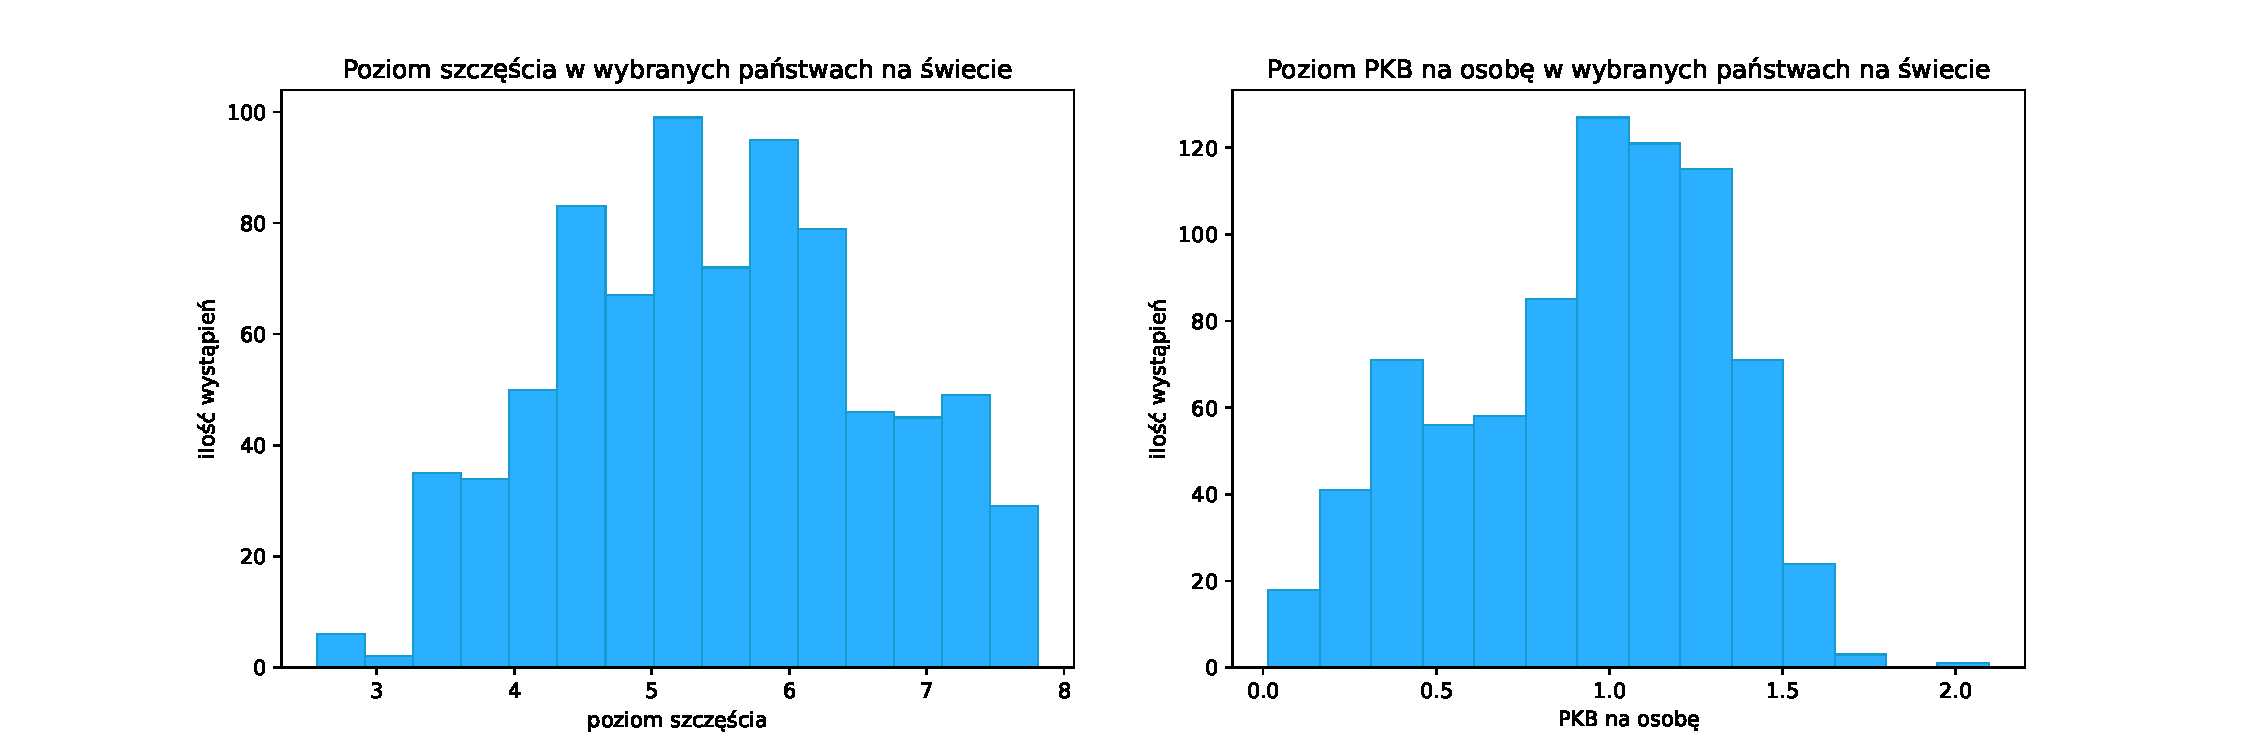
\includegraphics[scale=0.43]{hist.pdf}
		\caption{Histogramy}
		\label{fig:hist}
	\end{center}
\end{figure}

Dystrybuanty empiryczne [\ref{fig:distr}] pokazują z jakim prawdopodobieństwem natrafimy na kolejno szczęście i PKB mniejsze bądź równe od danej wartości. Gdy spojrzymy na dystrybuantę szczęścia, przypomina ona dystrybuantę rozkładu normalnego, o wariancji większej niż wariancja standardowego rozkładu normalnego. W przypadku dystrybuanty PKB, również przypomina ona rozkład normalny, z przesuniętą średnią. 

\begin{figure}[H]
	\begin{center}
		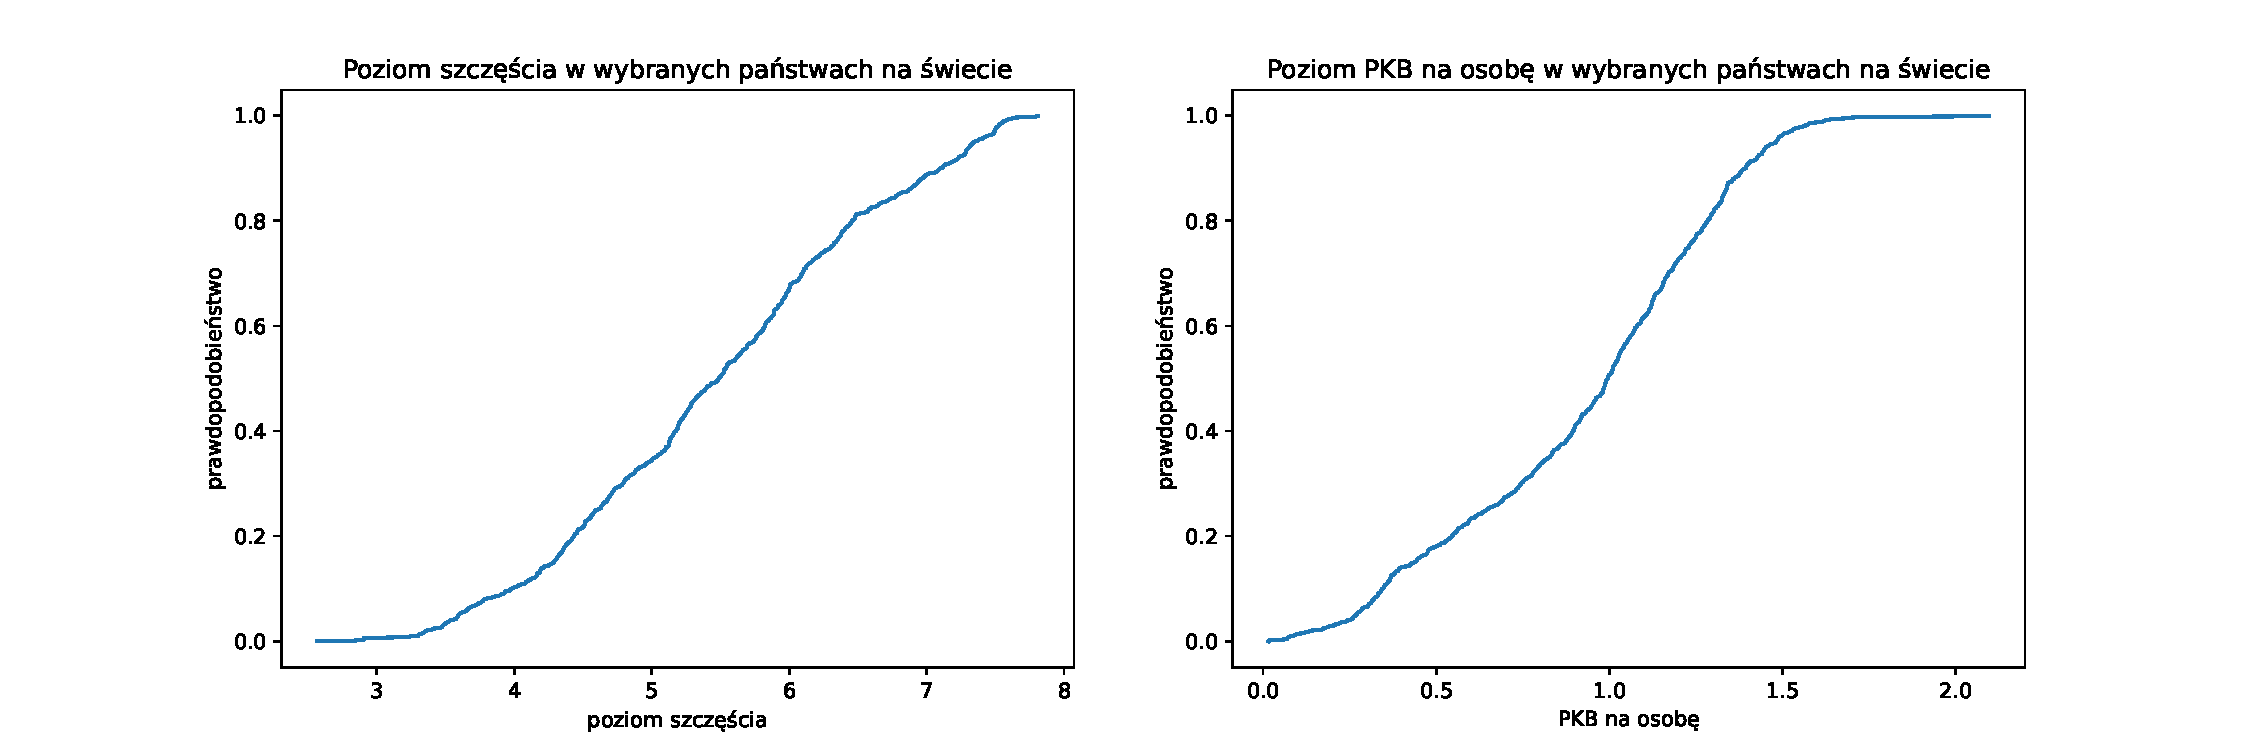
\includegraphics[scale=0.43]{distr.pdf}
		\caption{Dystrybuanta empiryczna}
		\label{fig:distr}
	\end{center}
\end{figure}

Wykres pudełkowy (ang. \textit{boxplot}) [\ref{fig:box}] jest to graficzna reprezentacja mediany oraz kwartyli. Wąsy mają długość półtorej wartości rozstępu międzykwartylowego. Co ciekawe, w naszych danych nie pojawiły się wartości odstające, zatem możemy sądzić, że dane zostały rzetelnie zebrane a ryzyko przeprowadzenia błędnej analizy (nieodzwierciedlającej rzeczywistych trendów) jest mniejsze.

\begin{figure}[H]
	\begin{center}
		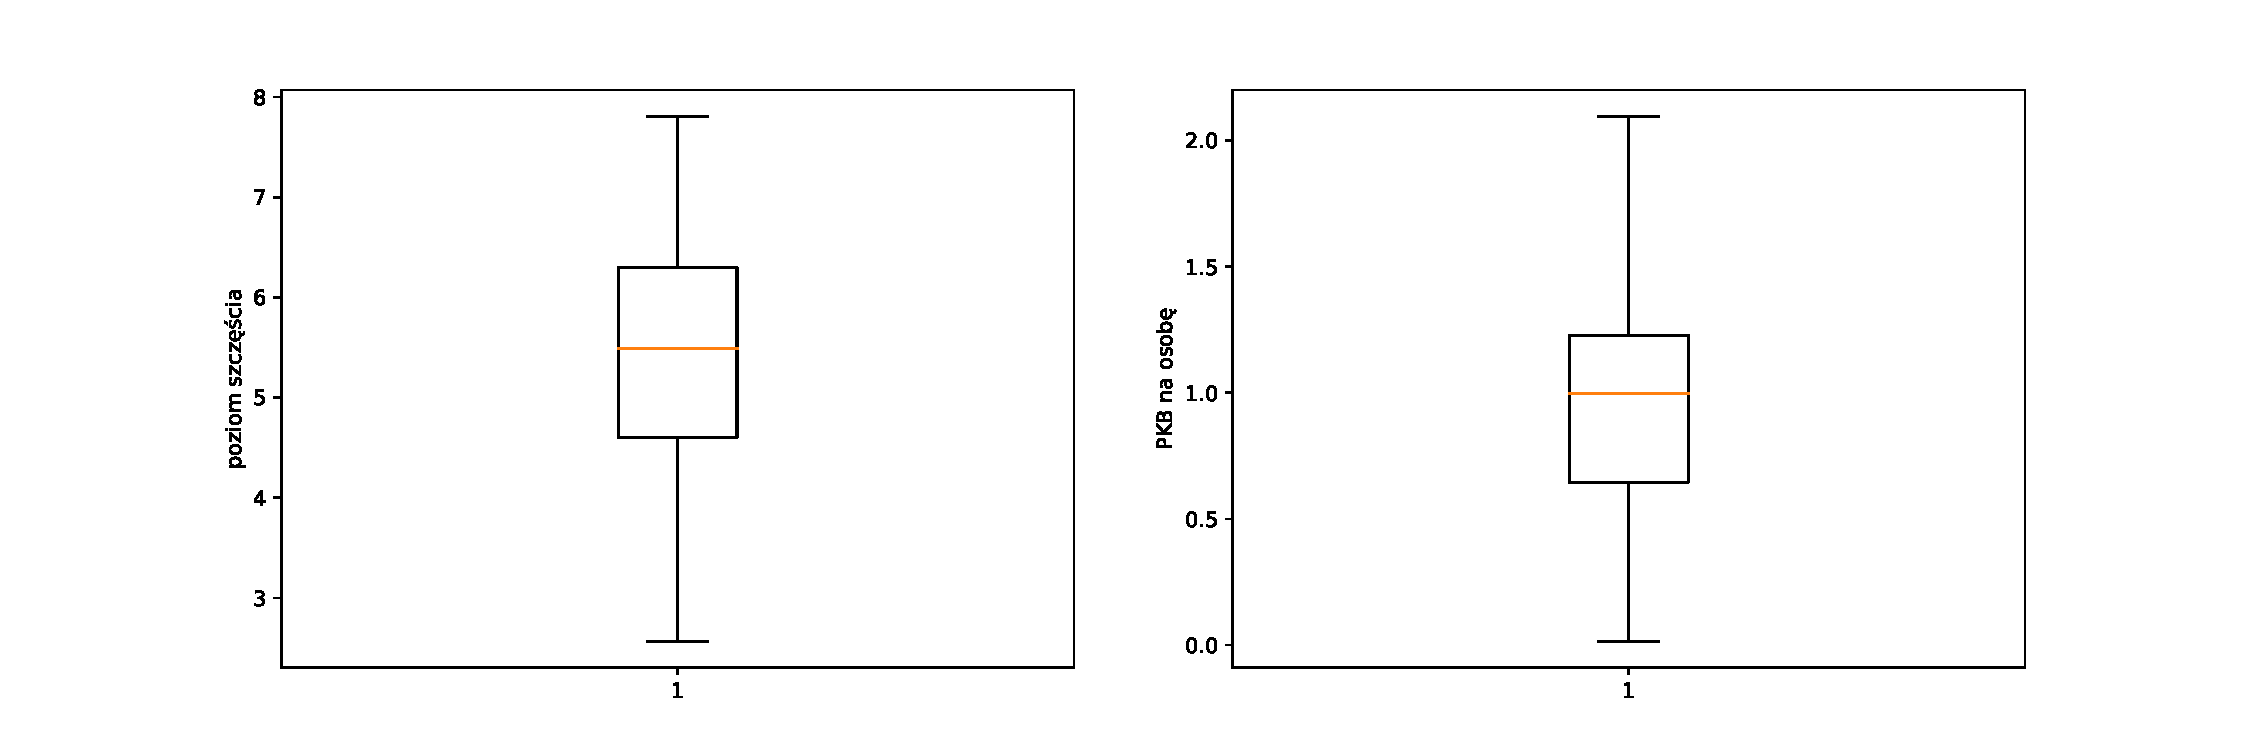
\includegraphics[scale=0.43]{box.pdf}
		\caption{Boxploty}
		\label{fig:box}
	\end{center}
\end{figure}

W tabeli [\ref{table}] podsumowałyśmy najistotniejsze miary położenia, rozproszenia, spłaszczenia i skośności. Rzeczwiście skośność którą odczytałyśmy z histogramu dla PKB jest ujemna (zatem rozkład jest lewoskośny), natomiast skośność dla szczęścia jest niewielka. Przypuszczenia z wykresu dystrybuanty empirycznej również się sprawdziły - wariancja szczęścia jest większa od jeden. 



\begin{table}[H]
	\centering
	\begin{tabular}{|ll|l|l|}
		\hline
		\rowcolor[HTML]{C0C0C0} 
		\multicolumn{2}{|l|}{\cellcolor[HTML]{C0C0C0}Miary}                             & Poziom szczęścia & PKB na osobe \\ \hline
		\multicolumn{1}{|l|}{}                               & średnia arytmetyczna     & 5.47             & 0.93         \\ \cline{2-4} 
		\multicolumn{1}{|l|}{}                               & średnia geometryczna     & 5.23             & 0.58         \\ \cline{2-4} 
		\multicolumn{1}{|l|}{}                               & średnia harmoniczna      & 5.35             & 0.81         \\ \cline{2-4} 
		\multicolumn{1}{|l|}{}                               & średnia ucinana 10\%     & 5.47             & 0.94         \\ \cline{2-4} 
		\multicolumn{1}{|l|}{}                               & mediana Q2               & 5.48             & 0.99         \\ \cline{2-4} 
		\multicolumn{1}{|l|}{}                               & Q1                       & 4.59             & 0.64         \\ \cline{2-4} 
		\multicolumn{1}{|l|}{położenia}    & Q3                       & 6.30             & 1.22         \\ \hline
		\multicolumn{1}{|l|}{}                               & rozstęp                  & 5.24             & 2.08         \\ \cline{2-4} 
		\multicolumn{1}{|l|}{}                               & rozstęp międzykwartylowy & 1.70             & 0.58         \\ \cline{2-4} 
		\multicolumn{1}{|l|}{}                               & wariancja nieobciążona   & 1.26             & 0.14         \\ \cline{2-4} 
		\multicolumn{1}{|l|}{}                               & odchylenie standardowe   & 1.12             & 0.38         \\ \cline{2-4} 
		\multicolumn{1}{|l|}{rozproszenia} & współczynnik zmienności  & 20.52            & 41.33        \\ \hline
		\multicolumn{1}{|l|}{spłaszczenia}                   & kurtoza                  & 2.25             & 2.31         \\ \hline
		\multicolumn{1}{|l|}{skośności}                      & skośność                 & -0.01            & -0.36        \\ \hline
	\end{tabular}
\caption{\label{table}Zestawienie statystyk.}
\end{table}
	
\section{Analiza zależności liniowej pomiędzy zmienną zależną a zmienną niezależną}

\begin{figure}[H]
	\begin{center}
		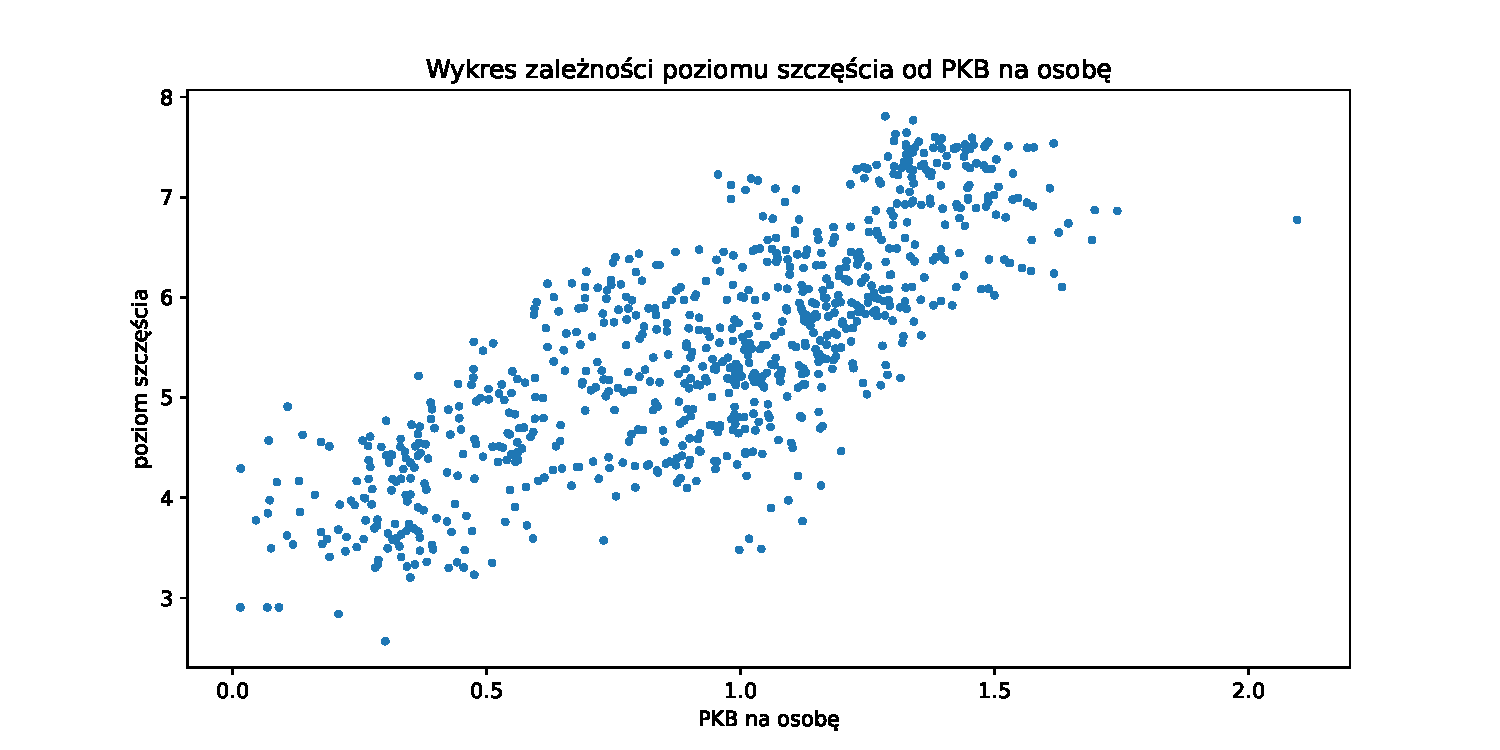
\includegraphics[scale=0.43]{plot1.pdf}
		\caption{p1}
		\label{fig:plot1}
	\end{center}
\end{figure}

\begin{figure}[H]
	\begin{center}
		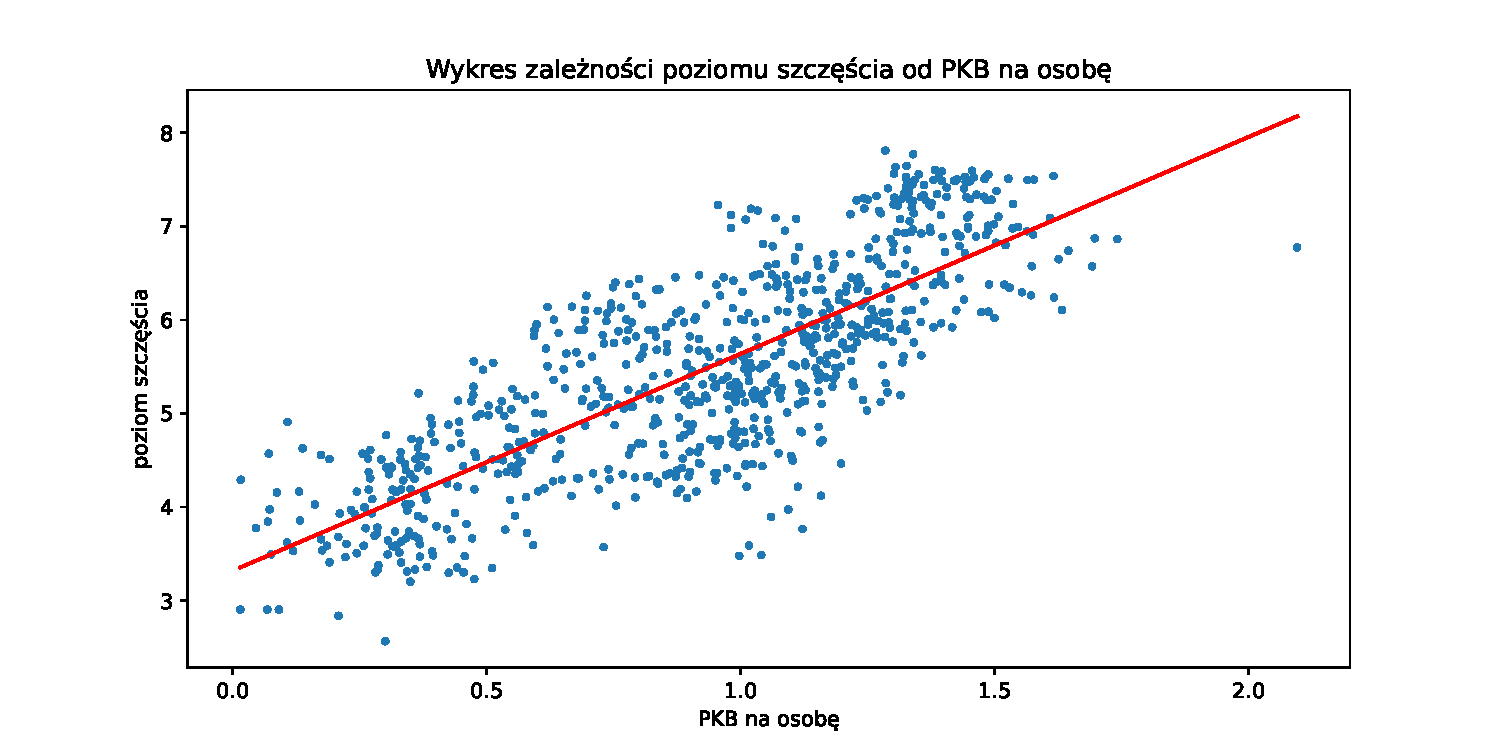
\includegraphics[scale=0.43]{plot2.pdf}
		\caption{p2}
		\label{fig:plot2}
	\end{center}
\end{figure}
	
\section{Analiza residuów}

\begin{figure}[H]
	\begin{center}
		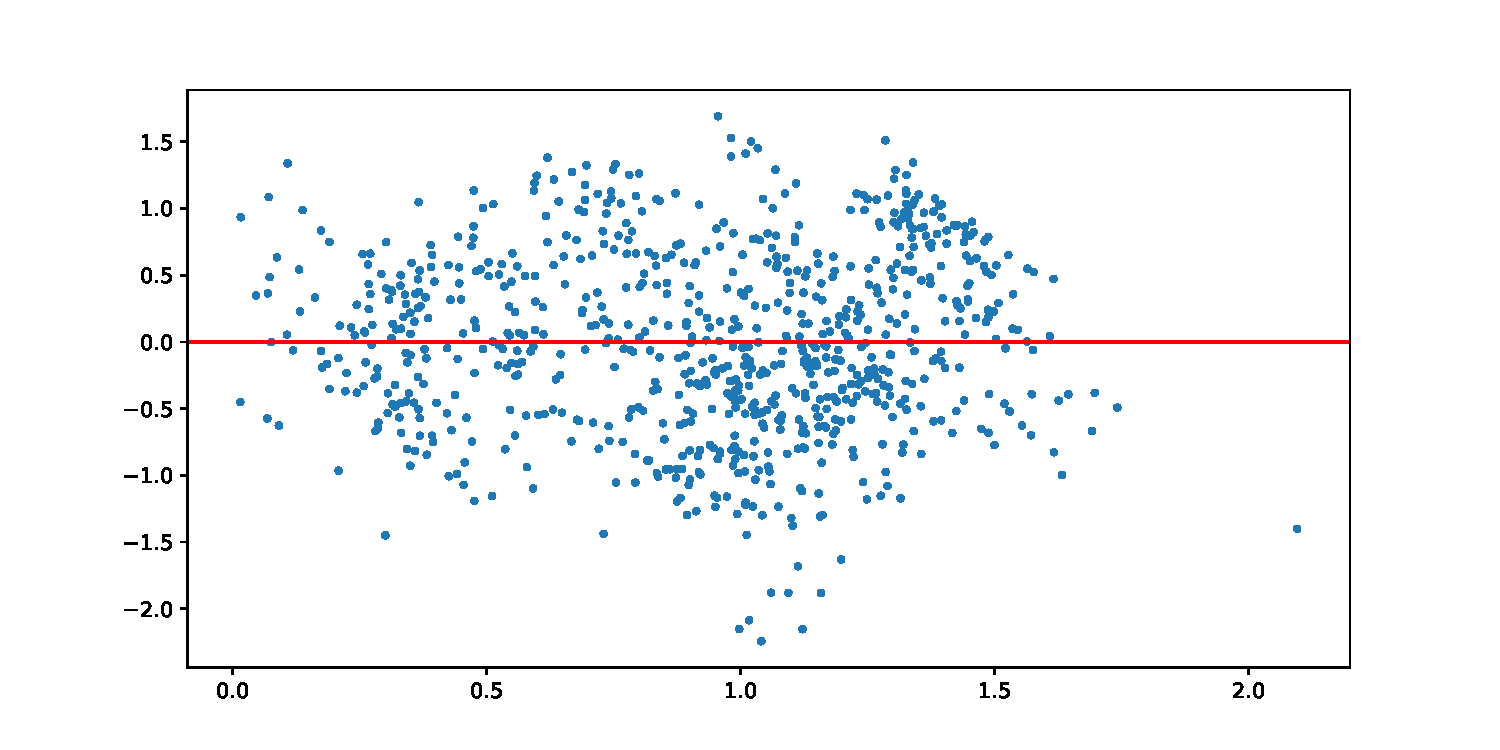
\includegraphics[scale=0.43]{res.pdf}
		\caption{Wy}
		\label{fig:res}
	\end{center}
\end{figure}

\begin{figure}[H]
	\begin{center}
		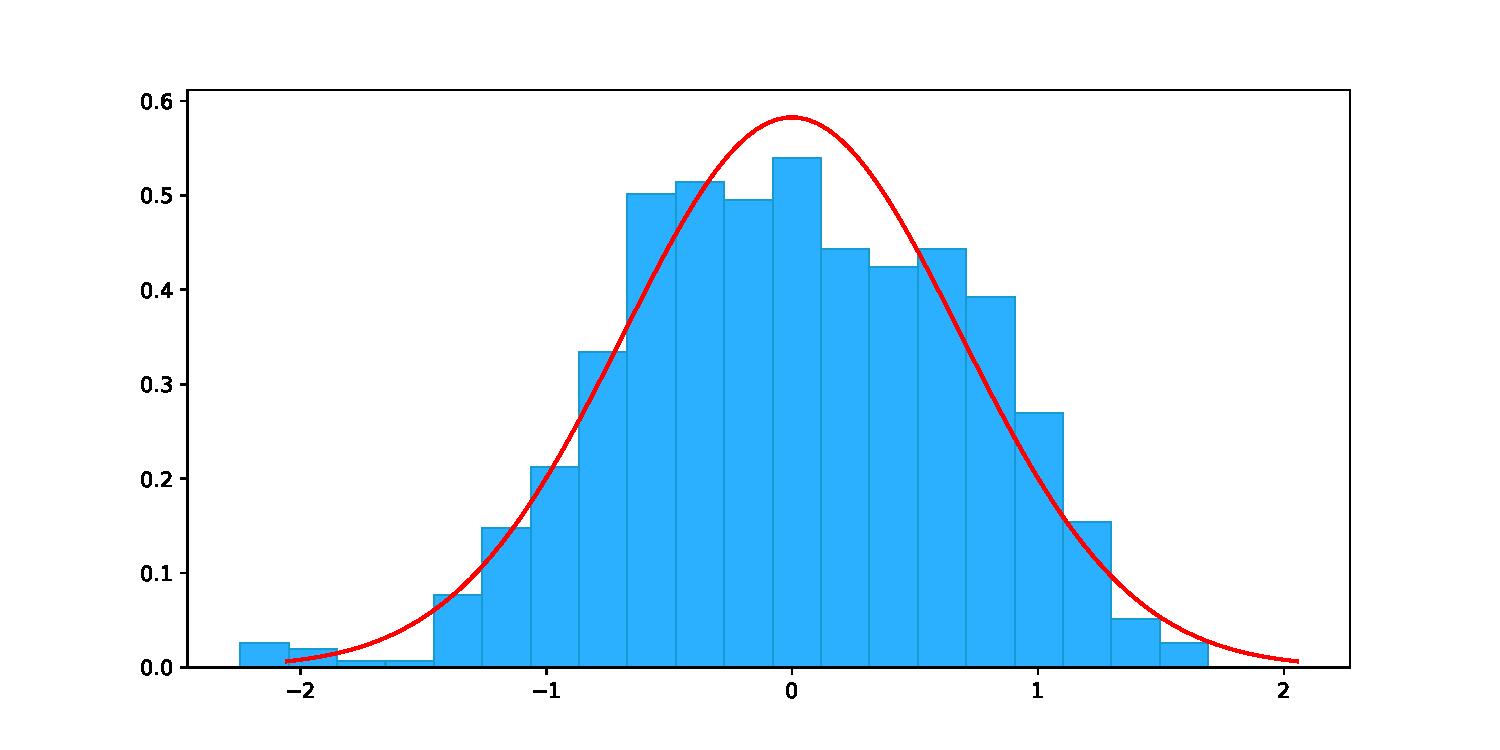
\includegraphics[scale=0.43]{res_hist.pdf}
		\caption{Wy}
		\label{fig:res_hist}
	\end{center}
\end{figure}

	
\section{Podsumowanie}
	Analizując przedstawione w raporcie statystyki możemy sformułować następujące wnioski i przypuszczenia dotyczące długości ogonów w populacji myszołowów rdzawosternych. Z histogramu widzimy, że badany rozkład przypomina rozkład normalny, jednak po obliczeniu skośności okazuje się, że różni się ona od skośności rozkładu normalnego, która wynosi zero. Podejrzewamy, iż może to być spowodowane licznością próby. Statystyczny myszołów rdzawosterny powinien mieć ogon o długości od $207,638$ do $236.66$ mm, (średnia arytmetyczna $\pm$ odchylenie standardowe). Biorąc średnią z populacji przewidujemy długość około $222,15$ mm. Wartości skrajne nie wpływają znacząco na wartość średniej - wiemy to po obliczeniu średniej Winsorowskiej ($222,182$ mm) i ucinanej ($222,104$ mm). 
	
	\section{Źródła}
	\begin{itemize}
		\item Wykłady
		\item \url{https://vincentarelbundock.github.io/Rdatasets/csv/Stat2Data/HawkTail.csv}
		\item \url{https://www.geo.fu-berlin.de/en/v/soga/Basics-of-statistics/Descriptive-Statistics/Measures-of-Position/index.html}
		\item \url{https://www.investopedia.com/terms/w/winsorized_mean.asp}
	\end{itemize}
	
	
\end{document}